\documentclass[a4paper,12pt]{extarticle}
\usepackage[utf8x]{inputenc}
\usepackage[T1,T2A]{fontenc}
\usepackage[russian]{babel}
\usepackage{hyperref}
\usepackage{indentfirst}
\usepackage{listings}
\usepackage{color}
\usepackage{xcolor}
\usepackage{here}
\usepackage{array}
\usepackage{multirow}
\usepackage{graphicx}
\usepackage{amsmath}

\hypersetup{
    colorlinks = false,
    linkbordercolor = {white}
}

\definecolor{string}{HTML}{B40000} % цвет строк в коде
\definecolor{comment}{HTML}{008000} % цвет комментариев в коде
\definecolor{keyword}{HTML}{1A00FF} % цвет ключевых слов в коде
\definecolor{morecomment}{HTML}{8000FF} % цвет include и других элементов в коде
\definecolor{сaptiontext}{HTML}{FFFFFF} % цвет текста заголовка в коде
\definecolor{сaptionbk}{HTML}{999999} % цвет фона заголовка в коде
\definecolor{bk}{HTML}{FFFFFF} % цвет фона в коде
\definecolor{frame}{HTML}{999999} % цвет рамки в коде
\definecolor{brackets}{HTML}{B40000} % цвет скобок в коде

\usepackage{caption}
\renewcommand{\lstlistingname}{Программа} % заголовок листингов кода

\bibliographystyle{ugost2008ls}

\usepackage{listings}
\lstset{ %
	extendedchars=\true,
	keepspaces=true,
	language=Python,						% choose the language of the code
	% Цвета
	keywordstyle=\color{keyword}\ttfamily\bfseries,
	%stringstyle=\color{string}\ttfamily,
	stringstyle=\ttfamily\color{red!50!brown},
	commentstyle=\color{comment}\ttfamily\itshape,
	morecomment=[l][\color{morecomment}]{\#},
	basicstyle=\footnotesize,		% the size of the fonts that are used for the code
	numbers=left,					% where to put the line-numbers
	numberstyle=\footnotesize,		% the size of the fonts that are used for the line-numbers
	stepnumber=1,					% the step between two line-numbers. If it is 1 each line will be numbered
	numbersep=5pt,					% how far the line-numbers are from the code
	backgroundcolor=\color{white},	% choose the background color. You must add \usepackage{color}
	showspaces=false				% show spaces adding particular underscores
	keywordstyle=color{blue}\bfseries, 
	showstringspaces=false,			% underline spaces within strings
	showtabs=false,					% show tabs within strings adding particular underscores
	frame=single,          		% adds a frame around the code
	tabsize=2,						% sets default tabsize to 2 spaces
	captionpos=t,					% sets the caption-position to top
	breaklines=true,				% sets automatic line breaking
	breakatwhitespace=false,		% sets if automatic breaks should only happen at whitespace
	escapeinside={\%*}{*)},			% if you want to add a comment within your code
	postbreak=\raisebox{0ex}[0ex][0ex]{\ensuremath{\color{red}\hookrightarrow\space}},
	texcl=true,
	inputpath=listings,                     % директория с листингами
}

\usepackage[left=2cm,right=2cm,
top=2cm,bottom=2cm,bindingoffset=0cm]{geometry}

%% Нумерация картинок по секциям
\usepackage{chngcntr}
\counterwithin{figure}{section}
\counterwithin{table}{section}

%%Точки нумерации заголовков
\usepackage{titlesec}
\titlelabel{\thetitle.\quad}
\usepackage[dotinlabels]{titletoc}

%% Оформления подписи рисунка
\addto\captionsrussian{\renewcommand{\figurename}{Рисунок}}
\captionsetup[figure]{labelsep = period}

%% Подпись таблицы
\DeclareCaptionFormat{hfillstart}{\hfill#1#2#3\par}
\captionsetup[table]{format=hfillstart,labelsep=newline,justification=centering,skip=-10pt,textfont=bf}

%% Путь к каталогу с рисунками
\graphicspath{{fig/}}

\begin{document}	% начало документа
\counterwithin{lstlisting}{section}

% Титульная страница
%\begin{titlepage}	% начало титульной страницы

	\begin{center}		% выравнивание по центру

		Санкт-Петербургский Национально Исследовательский Университет\\
		информационных технологий, механики и оптики \\
		Кафедра систем управления и информатики\\[3cm]
		% название института, затем отступ 6см
		
		\huge \textbf{РЕФЕРАТ}\\[0.5cm]
		\large Электромеханические системы\\[0.1cm]
		\large Система автоматического управления квадракоптера Parrot ARDrone 2.0\\[2cm]

	\end{center}


	\begin{flushright} % выравнивание по правому краю
%		\begin{minipage}{0.5\textwidth} % врезка в половину ширины текста
%			\begin{flushleft} % выровнять её содержимое по левому краю

				\large Выполнили студенты группы P3335\\
				\large А.М. Зенкин\\[0.5cm]
				\large К.В. Карпов\\[0.5cm]
				
				\large Принял  к.т.н., доцент кафедры СУиР\\
				\sign[4cm]\large  М.С. Чежин\\
				\large Оценка: \sign\\
				«\underline{\hspace{0.7cm}}» \underline{\hspace{2cm}} \the\year г.

%			\end{flushleft}
%		\end{minipage}
	\end{flushright}
	
	\vfill % заполнить всё доступное ниже пространство

	\begin{center}
	\large Санкт-Петербург\\
	\large \the\year % вывести дату
	\end{center} % закончить выравнивание по центру

\thispagestyle{empty} % не нумеровать страницу
%\end{titlepage} % конец титульной страницы
\newpage


% Содержание
% Содержание
\renewcommand\contentsname{\centerline{Содержание}}
\tableofcontents
\thispagestyle{fancy}
\newpage



\section*{Введение}

В наши дни все большую популярность набирают беспилотные летательные аппараты, а именно мультикоптеры или, как их чаще всего называют, квадрокоптеры - это летательный аппарат построенный по вертолётной схеме с тремя и более несущими винтами. Обычно данные устройства имеют грузоподъемность от 500г до 2-3 кг, что позволяет поднять в воздух небольшую фото или видеокамеру (обычно экшн-камера в более дешёвых моделях, либо зеркальные камеры в профессиональных). Но сейчас всё больше и больше начинают использовать квадрокоптеры в технических сферах, например, для построения карты местности, используя монокулярную камеру или слежения за выбранным объектом. В связи с этим в интернете появляется довольно много материала по данной тематике, так как это с одной стороны занимательная, а с другой достаточно перспективная отрасль. Как следствие всего вышесказанного, была поставлена задача стабилизации квадрокоптера в заданной точке пространства, облёт препятствия, слежение за выбранным объектом и построение 3D карты местности используя S.L.A.M. В данной работе необходимо подобрать непосредственно сам квадрокоптер и рассмотреть возможную систему автоматического управления+ беспилотным летательным аппаратом.
\addcontentsline{toc}{section}{Введение}

\newpage

\section{Обзор литературы по области применения САУ}

В настоящее время квадрокоптеры используются в самых различных сферах. Рассмотрим некоторые отрасли применения квадрортора и его разновидности.
В настоящее время существуют следующие классы квадрокоптеры
\subsubsection{Микро класс}
Начнем с самых маленьких представителей данных БЛА. И первым таким представителем является DHD D1. Самый маленький на сегодняшний день квадрокоптер, который умещается в ладонь.  Создан в основном для развлечений, но также можно приобрести базовае знания об управлении коптерами.\cite{geek}
\subsubsection{Меленький класс}
Переходим к следующему квадрокоптеру – старшему брату для нашего DHD D1 – Eachine H8 Mini. С его помощью уже можно ощутить вес квадрокоптера. Как можно заметить, на данной игрушке уже установлены защитные ограничители для лопастей, а это значит, что повреждений от такого квадрокоптера ( а точнее, от его винтов) ждать практически не придется. Дальность действия всего 30 метров, но для дома этого вполне хватит. Еще немного больше в размере, и стабильнее в полете. Размер такого квадротора около 170 мм.\cite{geek}
\subsubsection{250 класс}
Размер такого аппарата уже около 250 мм по диагонали. Хочу заметить, что диагональ коптера именно от двигателя до двигателя и защита пропеллеров сюда не входит. Данная модель не только способна летать в хорошую (а именно практически безветренную) погоду, но и вдобавок может доставить дополнительное удовольствие, т.к. на ней установлена миниатюрная камера. Однако радиус действия так же ограничен и составляет около 50 м. Для улицы это, конечно, немного, но на первое время как раз.\cite{geek}
\subsubsection{350 класс}
Данная модель уже оснащена камерой и способена транслировать видео прямо на ваш смартфон. Однако дальность действия управления также ограничена 50 м. Также ждать качества от стандартной камеры не стоит. Кроме того, камера на таких моделях крепится на жесткий кронштейн, поэтому стабилизации ждать не приходиться.\cite{geek}
\subsubsection{450 класс}
Класс обладает самой ремонтноспособной рамой. Также данный коптер лучше сопротивляется ветру чем 350-ый и более мелкие классы. Единственный минус – в рюкзак его уже не положить. Ну и комплектовать оборудованием для видеосъемки придется самому. В готовых вариантах такие дроны не продаются. В основном такие коптеры используются для камер GoPro и аналогов.\cite{geek}
\subsubsection{550-700 класс}
Классы от 550 до 700 вполне способны носить на борту небольшие зеркальные фотокамеры типа Sony nex 5n и аналогов с подвесами для стабилизации. Но тут в основном идут варианты с самостоятельной сборкой. За основу же например можно взять рамы Tarot 680, а остальное подбирать на основе ваших предпочтений.\cite{geek}

Вот основные классы коптеров на сегодняшний день. Говорить о ценах на каждый из данных истройств не имеет смысла, т.к. все зависит от того, что вы хотитет установить на свой БЛА и какой бренд вы собираетесь выбрать.\cite{geek}

\section{Объект управления САУ и его технические
характеристики}

\subsection{Объект управления САУ}
Квадрокоптер Parrot AR.Drone 2.0 — представитель класса любительских квадрокоптеров небольших размеров, который предназначен для полета на небольшие расстояния в открытой местности, а также для использования данного беспилотного летательного аппарата, далее бла, в домашних условиях. Управлять дроном можно с любого устройства, поддерживающего wifi, для начинающих пользователей предусмотрено приложение на смартфоны - AR.FreeFlight, который ограничевает функционал, но позволяет немедленно приступить к непосредственному использованию данного бла без особых усилий. Дрон оснащен целым рядом встроенных датчиков и контроллером, которые позволяют стабилизировать квадрокоптер во время полета. Также для данного бла компания Parrot, как и для остальных своих продуктов, поставляет открытую библиотеку - SDK2.0, которая позволяет пользователю напрямую программироать дрон. Поэтому он стал достаточно популярной исследовательской платформой для компьютерного зрения и робо разведки.

\subsection{Технические характеристики САУ}

Технические характреистики квадрокоптера приведены в таблице \ref{tab:1}.\cite{Gurg}\cite{xak}\cite{Thes1}

\begin{table}[H]
\caption{\label{tab:1} Технические характеристики квадрокоптера ARDrone 2.0}
\begin{center}
\def\tabcolsep{10pt} %расстояние между словами по горизонтали
\def\arraystretch{1.23}% с этим тоже можно поигаться, чтобы луяше выглядело
\fontsize{13}{14}\selectfont %и это размеры шрифтов в таблице
\begin{tabular}{|c|c|}
\hline
Характеристика                                                                          & Описание                                                                                                                                                                                                            \\ \hline
\multicolumn{2}{|c|}{Электронное оснащение}                                                                                                                                                                                                                                                                   \\ \hline
Процессор                                                                               & \begin{tabular}[c]{@{}c@{}}Процессор: ARM Cortex A8 1 ГГц \\ 32-разрядный процессор \\ с видео DSP 800 МГц TMS320DMC64x\end{tabular}                                                                                \\ \hline
ОС                                                                                      & Linux 2.6.32                                                                                                                                                                                                        \\ \hline
ОЗУ                                                                                     & DDR2 1 ГБ при 200 МГц                                                                                                                                                                                               \\ \hline
USB                                                                                     & Высокоскоростной USB 2.0 для расширений                                                                                                                                                                             \\ \hline
Беспроводная связь                                                                      & Wi-Fi b g n                                                                                                                                                                                                         \\ \hline
Гироскоп                                                                                & 3 оси, точность 2000 °/ сек.                                                                                                                                                                                       \\ \hline
Акселерометр                                                                            & 3 оси, точность +/- 50 мг                                                                                                                                                                                           \\ \hline
Магнитометр                                                                             & 3 оси, точность 6 °                                                                                                                                                                                                 \\ \hline
Датчик давления                                                                         & Точность +/- 10 Па                                                                                                                                                                                                  \\ \hline
\begin{tabular}[c]{@{}c@{}}Ультрозвуковой\\  датчик высоты\end{tabular}                 & Измеряет высоту                                                                                                                                                                                                     \\ \hline
Вертикальная камера                                                                     & QVGA 60 FPS для измерения скорости движения                                                                                                                                                                         \\ \hline
\multicolumn{2}{|c|}{Запись HD-видео}                                                                                                                                                                                                                                                                         \\ \hline
\begin{tabular}[c]{@{}c@{}}Фронтальная\\ камера\end{tabular}                            & \begin{tabular}[c]{@{}c@{}}720p камера с разрешением 30 кадров в секунду\\ Широкоугольный объектив: диагональ 92 °\\ Основной профиль кодирования: H264\\ Формат фотографий: JPEG\\ Подключение: Wi-Fi\end{tabular} \\ \hline
\multicolumn{2}{|c|}{Двигатели и вес}                                                                                                                                                                                                                                                                         \\ \hline
Двигатели                                                                               & \begin{tabular}[c]{@{}c@{}}4 бесколлекторных двигателя типа «inrunner»\\  14,5 Вт и 28 500 об/мин\end{tabular}                                                                                                          \\ \hline
\begin{tabular}[c]{@{}c@{}}Микро шариковый \\ подшипник\end{tabular}                    & Да                                                                                                                                                                                                                  \\ \hline
\begin{tabular}[c]{@{}c@{}}Бронзовые самосмазывающиеся \\ шарикоподшипники\end{tabular} & Да                                                                                                                                                                                                                  \\ \hline
Вес с внутренней рамой                                                                  & 380 г                                                                                                                                                                                                               \\ \hline
Вес с внешней рамой                                                                     & 420 г                                                                                                                                                                                                               \\ \hline
\end{tabular}
\end{center}
\end{table}

\section{Принцип работы САУ и его функциональная схема}
\subsection{Принцип работы квадрокоптера}
Здесь все довольно просто, хотя, сложность устройства во многом зависит от его класса. В целом, схема одна – дрон представляет из себя устройство, состоящее из:\cite{kvadr}
\begin{itemize}
\item Центрального корпуса, в котором находится защищенная оболочкой электроника;
\item Рамы, на которой закрепляются пропеллеры;
\item Крепления для камеры, и, собственно, самой камеры.
\end{itemize}
Правда, последний пункт относится только к более продвинутым аппаратам.\\
Сбалансированность полета и хорошая управляемость дрона обеспечивается вращением пропеллеров в противоположные стороны – одна пара вращается по часовой стрелке, а одна – против нее.\\
С помощью пульта, человек может отдавать команды каждому из винтов, от чего и зависит, как квадрокоптер будет вести себя в воздухе:
\begin{itemize}
\item При вращении всех винтов с одной и той же скоростью, аппарат взлетает\cite{thes};
\item Если один из пропеллеров вращается быстрее, чем остальные – коптер наклоняется и начинает двигаться в соответствующую сторону;
\item Если одна пара пропеллеров начинает вращаться быстрее, квадрокоптер поворачивается в сторону.
\end{itemize}
Управления движениями квадрокоптера приведено на рисунке.\ref{pic:pic_2}.\cite{Parrot}
\begin{figure}[H]
	\begin{center}
		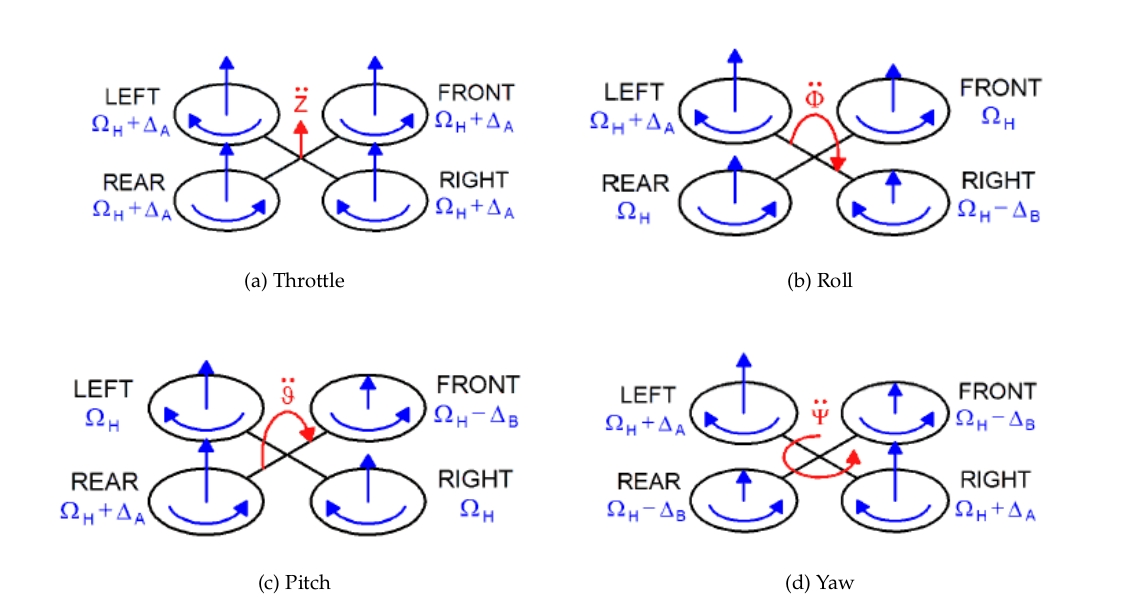
\includegraphics[scale=0.4]{pics/kren}
		\caption{- Движения квадрокоптера} 
		\label{pic:pic_2} % название для ссылок внутри кода
	\end{center}
\end{figure}
Маневры получаются путем изменения углов наклона, угла поворота и угла поворота вправо. Рисунок \ref{pic:pic_3}.\cite{Parrot}
\begin{figure}[H]
	\begin{center}
		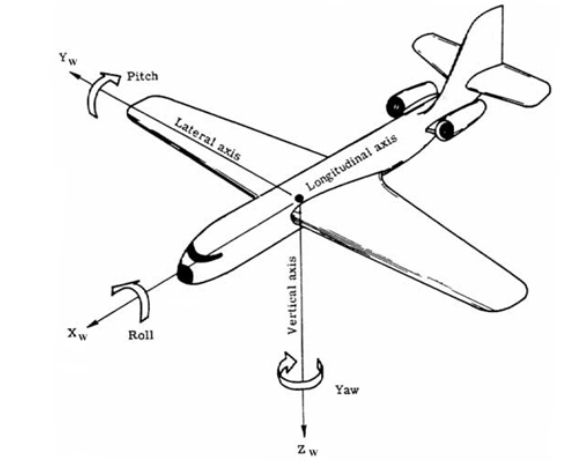
\includegraphics[scale=0.4]{pics/sam}
		\caption{- Маневры квадрокоптера} 
		\label{pic:pic_3} % название для ссылок внутри кода
	\end{center}
\end{figure}

\subsection{Функциональная схема и ее описание}
Функциональная схема квадрокоптера Parrot ARDrone 2.0 приведена на рисунке \ref{pic:pic_1}.

\begin{figure}[H]
	\begin{center}
		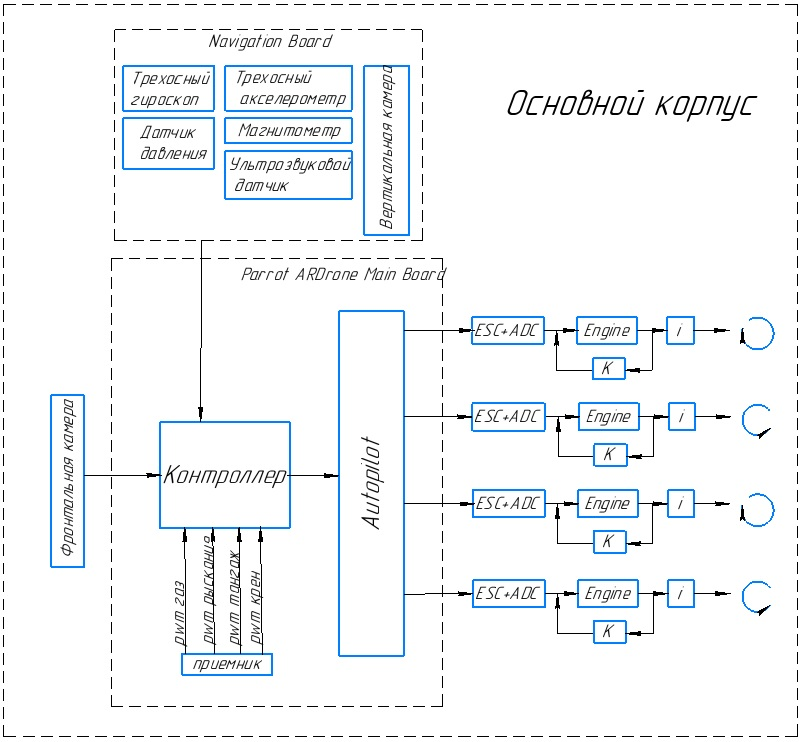
\includegraphics[scale=0.9]{pics/FunCxem}
		\caption{- функциональная схема} 
		\label{pic:pic_1} % название для ссылок внутри кода
	\end{center}
\end{figure}

\newpage

На материнской плате установлен контроллер и автопилот. Роль контроллера играет ARM Cortex A8 1 ГГц, 32-разрядный процессор с видео DSP 800 МГц TMS320DMC64x с операционной системой Linux 2.6.32                                                                                                                                

В роли платы навигации выступает Parrot AR.Drone Navigation Board PF070007AA, которая была специально ращработана компание Parrot для данного квадрокоптера. На нее установлены:
\begin{itemize}
\item Трехосный гироскоп( точность 2000 °/сек);
\item Трехосный акселерометр( точность +/- 50 мг);
\item Датчик давления( точность +/- 10 Па);
\item Магнитометр( точность $6^{\circ}$);
\item Ультрозвуковой датчик для измерения высоты до 5м( точность +/- 0.5 см);
\end{itemize}
Также в данном устройстве вертикальная камера отностися к плате навигации. Данная камера высчитывает оптический поток, на основе которого впоследствии высчитывается скорость квадрокоптера. Всё это необходимо для того, чтобы высчитывать одометрию, которая поступает на контроллер, а после на автопилот, где уже идет корректировка положения квадрокоптера.

На контроллере также установлен модуль Wifi, на который передаются данный о желаемом тангаже, газе, рысканье и крене. Подключить к нему может любое устройство, на котором установлен Wifi.

Аппарат приводится в движение четырьмя бесколлекторными 14.5 ваттными электродвигателями типа «inrunner» 28 500 об/мин, на котрых имеется обратная связь.

Мотор подсоединяется к электронному контроллеру, созданному компанией Parrot специально для AR.Drone 2.0, который контролирует скорость двигателя:
\begin{itemize}
\item ESC( англ - engine speed controller). 8-битный микроконтроллер низкого напряжения( 8 MIPS AVR CPU);
\item 10-битный аналогово-цифровой преобразователь
\end{itemize}

На каждый из четырех моторов установлен редуктор с шестернями из нилатрона, которые на выходе выдают скорость 3300 PRM.

В основном корпусе установлена фронтальная HD камера с углом обзора в $92^{\circ}$\cite{1}

\section{Основные элементы САУ и требования к
ним}

Квадрокоптер комнапии Parrot ARDrone 2.0 состоит из следующих элементов:\cite{zap}

\begin{itemize}
\item Основной корпус с камерой Parrot AR.Drone 2.0;
\item Материнская плата Parrot AR.Drone 2.0
\item Корпус для полётов в помещении Parrot AR.Drone 2.0 (с защитой лопастей)
\item Защита шестерней и двигателей квадрокоптера Parrot AR.Drone 2.0
\item Навигационная плата Parrot AR.Drone 2.0
\item Мотор Parrot AR.Drone 2.0
\item Плата для заряда батарей Parrot AR.Drone 2.0
\item Карбоновые пропеллеры для Parrot AR.Drone 2.0
\item Подшипники для Parrot AR.Drone 2.0
\item Набор цветных шестерней и валов Parrot AR.Drone 2.0 
\item Крестовина Parrot AR.Drone 2.0 
\item Аккумулятор повышенной ёмкости для Parrot AR.Drone 2.0 GiFi 2300 мАч
\end{itemize}

Особое внимание уделю элементу, осуществляющему преобразование электрической энергии в механическую. В данном квадрокоптере стоит 4 бесколлекторных двигателя типа «inrunner», который был специально расзаботан компанией Parrot для ARDrone 2.0, с мощностью в 14.5 Ватт, который может развить скорость в 28 500 об/мин. Скорость каждого из двигателей контролируется 8 битным контроллером в сочетании с 10 битный аналогово-цифровым преобразователем. Также непосредственно в самом двигателе имеется обратная связь.\cite{Parrot}\cite{hab}
Данные двигатели позволяют развивать максимальную скорость полёта — 18 км/ч.\cite{1}
\newpage 
\addcontentsline{toc}{section}{Заключение}
\section*{Заключение}
AR.Drone 2.0 компании Parrot является одним из самых доступных беспилотных летательных аппаратов на данный момент для осуществления S.L.A.M'a и изучения основ строения и управления квадрокоптерами. Также данный БЛА обладает открытой библиотекой - SDK 2.0, что позволяет производить все возможные настройки и улучшать точность стабилизации посредством усовершенствования ПИД регулятора и САУ в общем. Если брать во внимание растущую популярность квадракоптеров, то улучшение програмной и механической составляющей является очень перспективным направлением. Не смотря на все свои плюсы, квадротор имеет также и ряд минусов. Во-первых, это слишком малая грузоподъемность, которая ограничивается тремястами граммами. Во-вторых, достаточно небольшое время в полете, примерно 12 минут\cite{Parrot}, в реальности при наличии множества внешних воздействий это знаечние падает до 7 минут. 
В-третьих, чтобы достичь стабилизайции квадрокоптера в воздухе на протяжении всего полета необходимо приложить немало усилий и произвети дополнительные действия для более точной работы датчиков ARDrone 2.0. И это только одни из самых явных минусов. Но не смотря на это, данный квадрокоптер является одним из самых качественных продуктов в своей ценовой категории.
\newpage

\renewcommand\refname{Список использованных источников}
\addcontentsline{toc}{section}{Список использованных источников}
\bibliographystyle{utf8gost705u}  %% стилевой файл для оформления по ГОСТу
\bibliography{sources} 

%\renewcommand\refname{Список использованных источников}
%\bibliography{sources}
%\addcontentsline{toc}{section}{Список использованных источников}

\end{document}
